% This is "sig-alternate.tex" V2.0 May 2012
% This file should be compiled with V2.5 of "sig-alternate.cls" May 2012
%
% This example file demonstrates the use of the 'sig-alternate.cls'
% V2.5 LaTeX2e document class file. It is for those submitting
% articles to ACM Conference Proceedings WHO DO NOT WISH TO
% STRICTLY ADHERE TO THE SIGS (PUBS-BOARD-ENDORSED) STYLE.
% The 'sig-alternate.cls' file will produce a similar-looking,
% albeit, 'tighter' paper resulting in, invariably, fewer pages.
%
% ----------------------------------------------------------------------------------------------------------------
% This .tex file (and associated .cls V2.5) produces:
%       1) The Permission Statement
%       2) The Conference (location) Info information
%       3) The Copyright Line with ACM data
%       4) NO page numbers
%
% as against the acm_proc_article-sp.cls file which
% DOES NOT produce 1) thru' 3) above.
%
% Using 'sig-alternate.cls' you have control, however, from within
% the source .tex file, over both the CopyrightYear
% (defaulted to 200X) and the ACM Copyright Data
% (defaulted to X-XXXXX-XX-X/XX/XX).
% e.g.
% \CopyrightYear{2007} will cause 2007 to appear in the copyright line.
% \crdata{0-12345-67-8/90/12} will cause 0-12345-67-8/90/12 to appear in the copyright line.
%
% ---------------------------------------------------------------------------------------------------------------
% This .tex source is an example which *does* use
% the .bib file (from which the .bbl file % is produced).
% REMEMBER HOWEVER: After having produced the .bbl file,
% and prior to final submission, you *NEED* to 'insert'
% your .bbl file into your source .tex file so as to provide
% ONE 'self-contained' source file.
%
% ================= IF YOU HAVE QUESTIONS =======================
% Questions regarding the SIGS styles, SIGS policies and
% procedures, Conferences etc. should be sent to
% Adrienne Griscti (griscti@acm.org)
%
% Technical questions _only_ to
% Gerald Murray (murray@hq.acm.org)
% ===============================================================
%
% For tracking purposes - this is V2.0 - May 2012

\documentclass{sig-alternate}
\usepackage{acronym}
\usepackage{array}
\usepackage{caption}

\begin{document}

% acronym definitions
\newacro{SoP}{Sense of Presence}
\newacro{QoE}{Quality of experience}
\newacroplural{QoE}{Quality of experiences}

\newacro{QoS}{Quality of service}
\newacro{EEG}{electroencephalography}
\newacro{ECG}{electrocardiography}
\newacro{Resp.}{respiration}
\newacro{MOS}{Mean opinion scores}
\newacro{CI}{Confidence intervals}
\newacro{IL}{immersiveness level}
\newacroplural{IL}{immersiveness levels}
\newacro{EOG}{electrooculogram}
\newacro{EMG}{electromyogram}
\newacro{HRV}{heart rate variability}


%
% --- Author Metadata here ---
\conferenceinfo{ACM MM}{2015 , Brisbane, Australia}
%\CopyrightYear{2015} % Allows default copyright year (20XX) to be over-ridden - IF NEED BE.
%\crdata{0-12345-67-8/90/01}  % Allows default copyright data (0-89791-88-6/97/05) to be over-ridden - IF NEED BE.
% --- End of Author Metadata ---
%MDSP : 
\title{ Multimodal Dataset on the Sense of Presence \\using physiological signals}
%\subtitle{Using physiological signals}
%\titlenote{A full version of this paper is available as
%\textit{Author's Guide to Preparing ACM SIG Proceedings Using
%\LaTeX$2_\epsilon$\ and BibTeX} at
%\texttt{www.acm.org/eaddress.htm}}}

% For aesthetic reasons, we recommend 'three authors at a time'
% i.e. three 'name/affiliation blocks' be placed beneath the title.



\numberofauthors{1} 
\author{
%\alignauthor 
Anne-Flore Perrin, He Xu, Eleni Kroupi, Martin Rerabek, Touradj Ebrahimi \\
       \affaddr{Multimedia Signal Processing Group (MMSPG)}\\
       \affaddr{Ecole Polytechnique Federale de Lausanne (EPFL), Switzerland}\\
       \email{\normalsize \{name.surname\}@epfl.ch}
%% 1st. author
%\alignauthor Anne-Flore Perrin \\
%       \affaddr{Multimedia Signal Processing Group (MMSPG)}\\
%       \affaddr{Ecole Polytechnique Federale de Lausanne (EPFL)}\\
%       \affaddr{EPFL/STI/IEL/GR-EB, Station 11, CH-1015 Lausanne, Switzerland}\\
%       \email{anne-flore.perrin@epfl.ch}
%%% 2nd. author
%\alignauthor He Xu\\
%       \affaddr{Multimedia Signal Processing Group (MMSPG)}\\
%       \affaddr{Ecole Polytechnique Federale de Lausanne (EPFL)}\\
%       \affaddr{EPFL/STI/IEL/GR-EB, Station 11, CH-1015 Lausanne, Switzerland}\\
%       \email{he.xu@epfl.ch}
%%% 3rd. author
%\alignauthor Eleni Kroupi\\
%       \affaddr{Multimedia Signal Processing Group (MMSPG)}\\
%       \affaddr{Ecole Polytechnique Federale de Lausanne (EPFL)}\\
%       \affaddr{EPFL/STI/IEL/GR-EB, Station 11, CH-1015 Lausanne, Switzerland}\\
%       \email{eleni.kroupi@epfl.ch}
%%% 4th. author
%\alignauthor Martin Rerabek\\
%       \affaddr{Multimedia Signal Processing Group (MMSPG)}\\
%       \affaddr{Ecole Polytechnique Federale de Lausanne (EPFL)}\\
%       \affaddr{EPFL/STI/IEL/GR-EB, Station 11, CH-1015 Lausanne, Switzerland}\\
%       \email{martin.rerabek@epfl.ch}
%%% 5th. author
%\alignauthor Touradj Ebrahimi\\
%       \affaddr{Multimedia Signal Processing Group (MMSPG)}\\
%       \affaddr{Ecole Polytechnique Federale de Lausanne (EPFL)}\\
%       \affaddr{EPFL/STI/IEL/GR-EB, Station 11, CH-1015 Lausanne, Switzerland}\\
%       \email{touradj.ebrahimi@epfl.ch}
%% 6th. author
%\alignauthor Charles Palmer\\
%       \affaddr{Palmer Research Laboratories}\\
%       \affaddr{8600 Datapoint Drive}\\
%       \affaddr{San Antonio, Texas 78229}\\
%       \email{cpalmer@prl.com}
}
% There's nothing stopping you putting the seventh, eighth, etc.
% author on the opening page (as the 'third row') but we ask,
% for aesthetic reasons that you place these 'additional authors'
% in the \additional authors block, viz.
%\additionalauthors{Additional authors: John Smith (The Th{\o}rv{\"a}ld Group,
%email: {\texttt{jsmith@affiliation.org}}) and Julius P.~Kumquat
%(The Kumquat Consortium, email: {\texttt{jpkumquat@consortium.net}}).}
\date{30 April 2015}
% Just remember to make sure that the TOTAL number of authors
% is the number that will appear on the first page PLUS the
% number that will appear in the \additionalauthors section.

\maketitle
\begin{abstract}
Measuring the perceived sense of immersion of a set of videos with respect to content, quality, resolution and sound system, is not an easy task because of the subjectivity of the human perception. A way to express the overall perceived quality of a video is to assess the \ac{QoE}, especially the \ac{SoP}. 
The latter, not so explored, is the principle we would like to assess. To be independent of the human way to explicitly express feelings and experiences, the analysis is carried out using physiological signals such as \ac{EEG}, \ac{ECG} and respiration.
\\The aim pursued is the creation of a data set containing all the above-mentioned signals in order to study the \ac{SoP}. The analysis demonstrates that data set is well constructed and functional for the assessment of the \ac{SoP}.

\end{abstract}

%% A category with the (minimum) three required fields
%\category{H.4}{Information Systems Applications}{Miscellaneous}
%%A category including the fourth, optional field follows...
%\category{D.2.8}{Software Engineering}{Metrics}[complexity measures, performance measures]
%
%\terms{Theory}
%
%\keywords{ACM proceedings, \LaTeX, text tagging}

\acresetall
\section{Introduction}
[PARAGRAPH ON QoE]
As digital television technologies aim to provide higher quality multimedia experience, possibly with various \ac{QoS}, the \ac{SoP} should be investigated to understand its impact on the \ac{QoE}.

According to Sadowski \& Stanney (2002), the \ac{SoP} also called immersion level, whether physical or psychological in nature, allows the sense of belief that the user as left the real world and is now "present" in a virtual environment. The aim to create a database on the \ac{SoP} is to study the impact of an high immersiveness experience on the \ac{QoE}, especially during the visualization of a multimedia content.

Traditionally, the perceived quality of a multimedia content is measured thanks to subjective quality assessment, where perceived quality of selected visual stimuli is obtained from a number of subjects. The subjects have to explicitly rate the quality of each stimulus in a pre-defines rating scale. This procedure is replicated by directing the questionnaire on the immersivennes level experienced during a stimulus.

The expression way of each people is specific and for instance cultural and educational dependent. So that the subjective ratings contains a subjective bias. A valuable survey of the \ac{SoP} can not only rely on subjects subjective rates. Based on the  Kroupi results on the assessment of 2D vs 3D quality, subjects'biological signals such as brain activity (\ac{EEG}), heart activity (\ac{ECG}) and respiration are objective data adequate to assess the \ac{SoP} complementarily to the subjective rates.

This paper assesses the creation of a database representing the differences in users'experiences during low, middle and high immersivness level stimuli visualization through \ac{EEG}, and peripheral physiological signals including \ac{ECG} and respiration as well as subjective rates.

We conduct subjective experiments, in which various immersivness stimuli multimedia content were presented to users, and both explicit subjective ratings and implicit \ac{EEG} and physiological response were captured.
\\Then an investigation of the felt experience transcribed in the subjective ratings allows to associate some \ac{QoS} properties to the \ac{SoP}. Finally the construction of a subject-independent classification system distinguishing the various immersiveness levels of stimuli based on \ac{EEG} and/or peripheral physiological signals.

The remainder of this paper is organized as follows.
The next section describes how we conducted experiments to collect subjective ratings and physiological responses. Section 3 presents the results of subjective rating analysis and user-independent physiological classification. Finally, conclusion is given in Section 4. 
\section{Data Collection}

\subsection{Participants}
The eight females and the twelve males participants had from 18 to 30 years old (23 median and average years of age). The 20 subject were screened for correct visual acuity (no errors on 20/30 lines) and color vision using Snellen and Ishiara charts respectively. They all provided written consents forms. Before each experiment, oral instruction were provided to the participants to explain their tasks. Additionally, a training session was organized to allow participants to familiarize with the assessment procedure. The content shown in the training session was selected by experts viewers in order to include examples of all evaluated aspects.

\subsection{Audio-visual stimuli}
Video stimuli are coming from nine video sequences extracted from four open source movies published by the Blender Foundation (Big buck bunny, Elephant dream, Sintel and Tears of Steel)\footnote{$http://media.xiph.org/$}. A supplementary sequence content was chosen for the training session.
\\The one minutes selected video contents have the highest audio, spatial end temporal energy and are related to the scene cuts.
The twenty seven video stimuli shown during an experiment are the combination of the nine video content with the three levels of immersiveness described below.
\\Low, middle and high immersiveness level were defined respectively thanks to the audio sound system, the video quality\textbackslash level of compression and the resolution.
The table \ref{IL} illustrates the previous comment.

\begin{table}[h]
\begin{tabular}{ |c || c | c | c | }
   \hline	
   Immersive senario 	& Low 			& Middle 		& High \\
   \hline	
   Audio 				& No Audio 		& Stereo		& Surround \\
   Quality (QP) 		& 36 			& 20			& 20 \\
   Resolution			& SD			& HD			& UHD\\
   \hline	
 \end{tabular}
 \caption{immersiveness levels}
 \label{IL}
 \end{table}

The video stimuli order could impact the data and so the results. Thus the sessions are built to allow this study : The first session will display the video stimuli from the lowest immersiveness level stimuli to the ones with the highest level. The second session order is middle immersiveness level stimuli, followed by the low immersiveness level stimuli and then the high immersiveness level stimuli. The last session will display the video stimuli from the video with the highest immersiveness level to ones with the lowest.
Thus the study of the change of devices is allowed and besides these constraints, the video order is different for each volunteer, thanks to a pseudo-random function. 

\subsection{Monitor, sound system and environment}

Professional high-performance 4K/QFHD LCD reference 56-inch monitor Sony Trimaster SRM-L560\footnote{$http://pro.sony.com/bbsccms/assets/files/cat/mondisp/$ \newline $brochures/di0195\_srm1560.pdf$} was used to display video stimuli.
As recommended in \cite{ScreenD}, the viewing distance was set at 1.6H (H - Height of the screen).
The Altec Lansing 5.1 THX speaker system, super subwoofer was used as audio sound system.
The laboratory setup has been thought to prevent the influence of involuntary influence of external factors, thus the reproductibility of the results is ensured.

\subsection{Physiological signal acquisition}

To record the brain activity, a 256 electrodes net was placed at the standard position on the scalp. An EGI's Geodesic EEG System (GES) 300 was used to record, amplify, and digitized the EEG signals while the participants were watching the stimuli. The heart activity is stored thanks to two standard \ac{ECG} electrode placed on the lower left rib cage and the upper right clavicle. Two respiratory inductive plethysmography belts (thoracic and abdomen)register the respiration. All signals were recorded at 250 Hz.

\subsection{Experimental protocol}

The experiments consists of three sessions intersected by ten-minutes breaks in order to avoid subject fatigue and lack of attention. Nine video stimuli (coming from the nine sequences) were presented in each session leading to a total of 27 video stimuli, and thus, to a total of 27 trials. 
The order of the \ac{SoP} levels of the video stimuli is set as described below. For the first session, the three first stimuli have a low \ac{IL}, the three next a middle \ac{IL} and the three last ones a high \ac{IL}. Respectively for the second and third session the order of the \ac{IL} is middle, low, high and high, middle and low.
Each trial consisted of a ten-second baseline period and a stimulus period. The biosignals recorded during the baseline period were used to remove stimulus-unrelated variations from the signals obtained during the stimulus period.


During the baseline periods, the subjects were instructed to remain calm and focus on a 2D white cross on a black background presented on the screen in front of them. Once this baseline period was over, a video stimulus was pseudo-randomly selected and presented.
After the video sequence was over, the subjects were asked to provide their self-assessed ratings for the particular video sequence without any restriction in time, following the Absolute Category Rating (ACR) evaluation methodology \cite{ACRevaluation}.

Regarding the self-assessed ratings, subjects were asked to evaluate the video sequences in terms of five different aspects, namely interest in the video content, perceived video quality, interest in audio content, immersiveness level and surrounding awareness. A 9-point rating scale was used that ranged from 1 to 9, with 1 representing the lowest value, and 9 the highest value of each aspect. In particular, the two extremes (1 and 9) correspond to "low" and "high" for interest in video and audio content as well as the perceived video quality, "no immersion" and "full immersion" for the immersion level and "no conscience of my environment" and "full conscience of my environment" for the surrounding awareness.

Once a trial was over, the next baseline period was recorded and the next video sequence was pseudo-randomly selected and presented. The procedure was repeated until all 27 video stimuli were presented and rated. Although the experiments lasted for almost two hours, including the training and the set up, the subjects did not report fatigue.

An illustration of a session is presented figure \ref{session}.

\begin{figure}[!ht]
    \center
    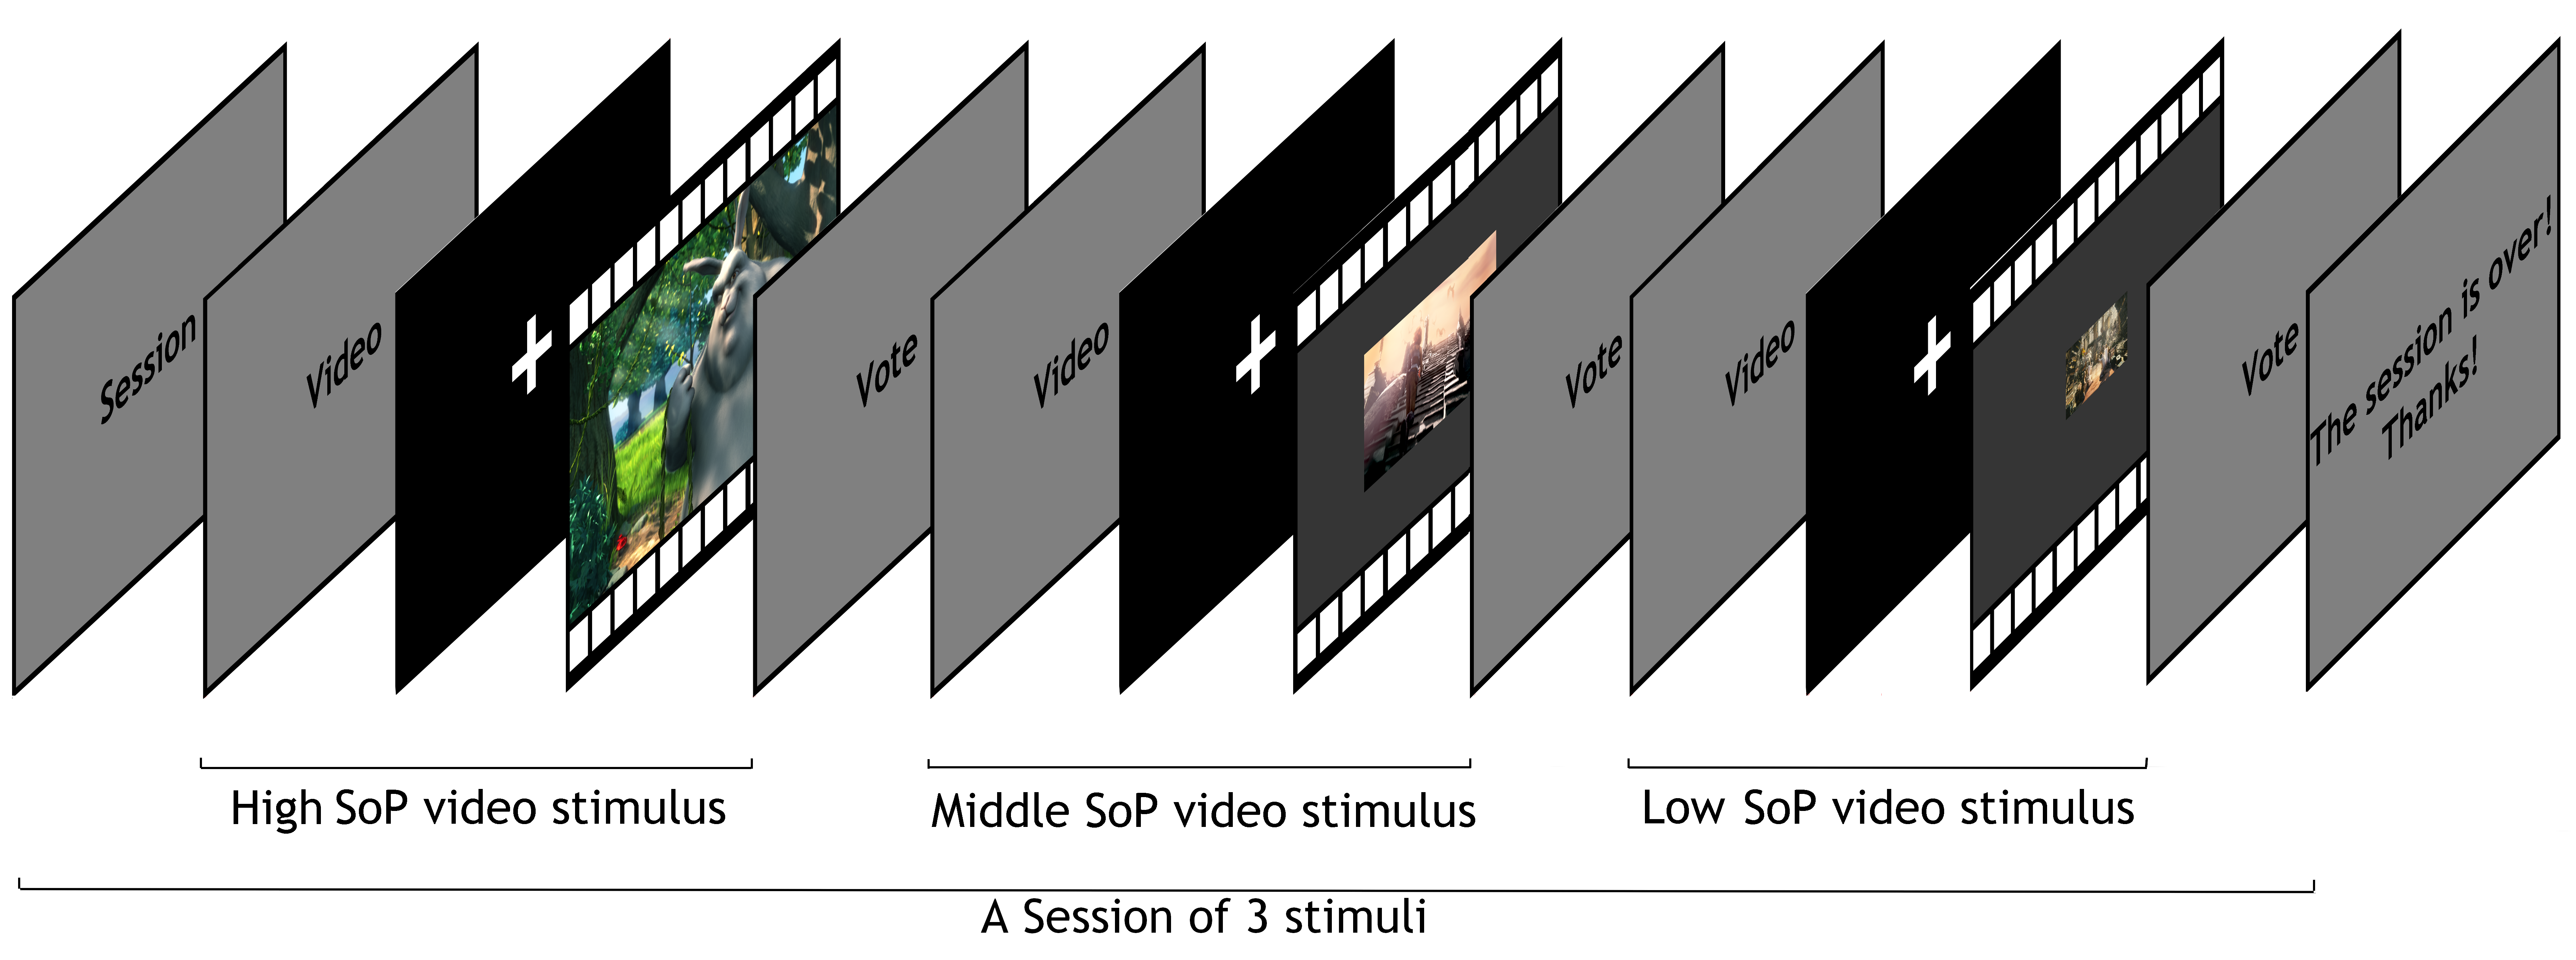
\includegraphics[width=0.5\textwidth]{./images/ExSession_.png}
    \caption{Example of a 3 video stimuli session progress }
    \label{session}
\end{figure}









 
%\input{ExperimentalProtocol} 
\section{Analysis}
The training session was used to illustrate the low, middle and high \ac{SoP} levels in order to guide subjects to bound their own perceived overall ratings more or less similarly.
To ensure that the ratings do not deviate significantly across subjects, the detection and elimination of outliers was performed.
The assessed \ac{IL} is the factor in which subjects were trained, thus the outliers detection was based on the scale of the perceived overall quality ratings. The outliers detection was applied according to the guidelines described in Section 2.3.1 of Annex 2 of \cite{Outliers}. In this study, no outliers were detected.

\subsection{Subjective ratings analysis}

The analysis conducted on the subjective rates includes score distribution histograms, box plots, \acf{MOS} and associated 95\% \acf{CI} and Pearson's correlations, assuming a Student's $t$-distribution of the subjective rates. 

The first verification is to ensure that all the \acfp{IL} were experienced by the subjects. The score distribution histogram of the ratings given by all the subjects for all the trials is presented in Figure \ref{Hist}. The value 1 corresponds to the lowest and 9 to the highest rate.

\begin{figure}[!ht]
    \center
    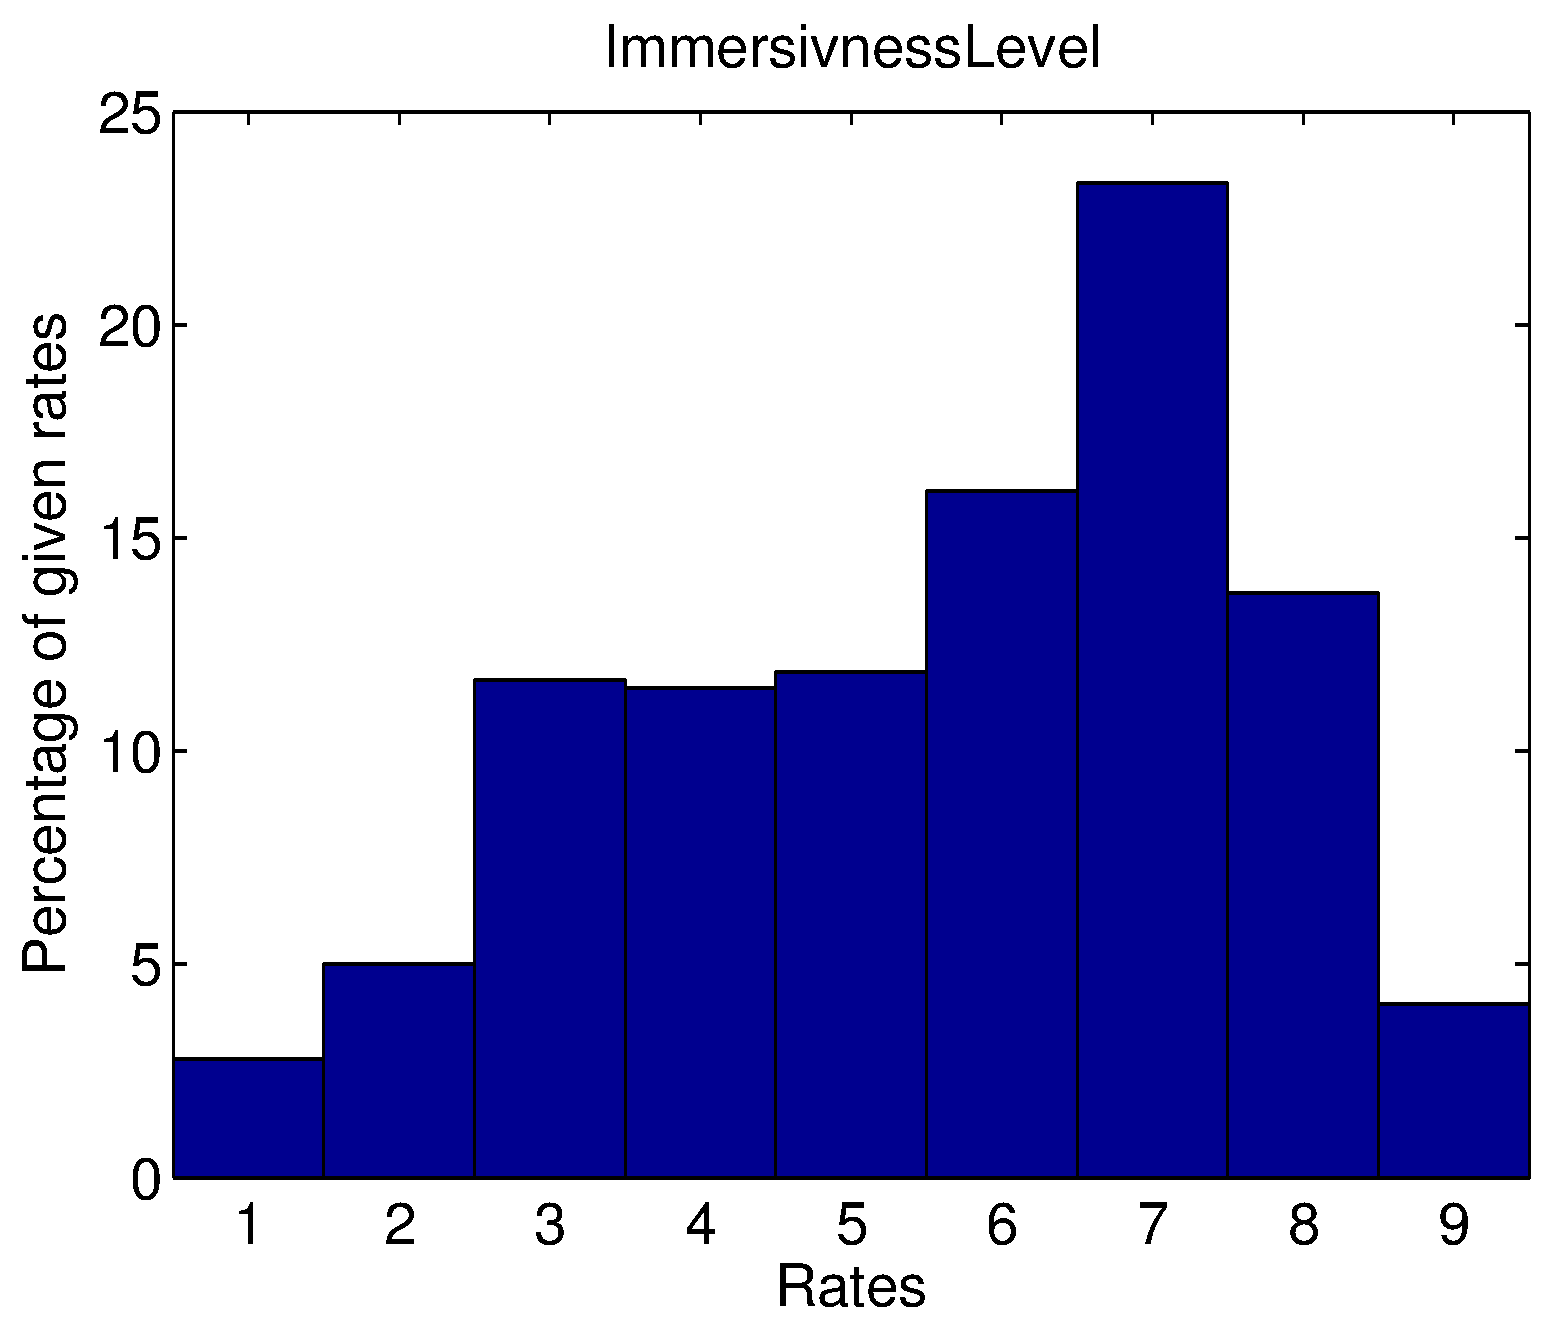
\includegraphics[width=0.3\textwidth]{./images/Hist9ImmersivnessLevel.png}
    \caption{Score distribution histogram for the \ac{IL} experienced }
    \label{Hist}
\end{figure}

As it can be observed, all the \ac{IL} were experienced during the experiments. More specifically, the distribution of the rates is roughly 20\% for the three lowest \ac{IL}, 40\% for the three middle and highest \ac{IL}. Thus the distribution almost describes three classes of immersiveness.  

\indent Figure \ref{MOS} shows the resulting \ac{MOS} and \ac{CI} for the \ac{SoP} experienced during stimuli.
\begin{figure}[!ht]
    \center
    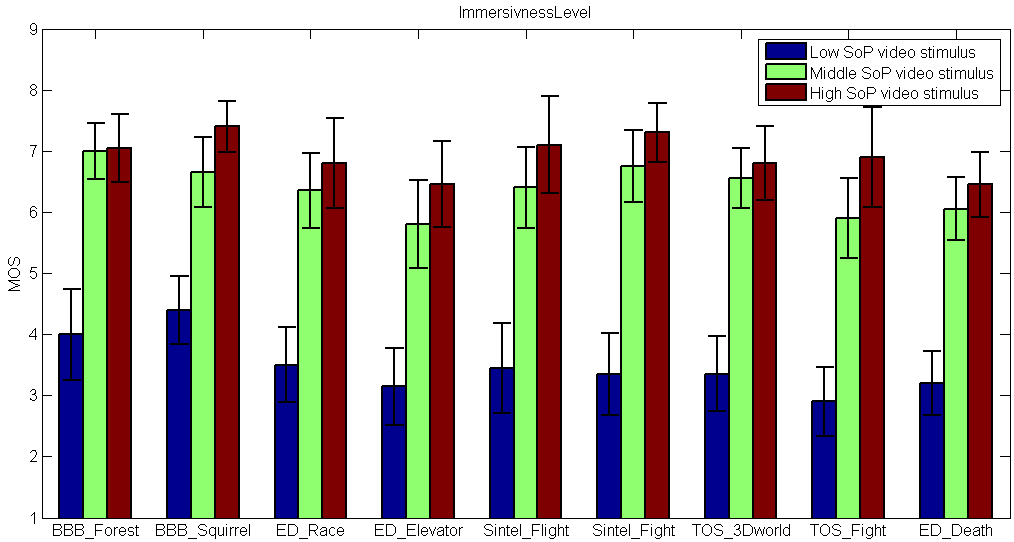
\includegraphics[width=0.45\textwidth]{./images/MOS_ImmersivnessLevel.png}
    \caption{\ac{MOS} and \ac{CI} for the \ac{IL} experienced}
    \label{MOS}
\end{figure}

The observed \ac{MOS} results valid the three \ac{IL} chosen during the experiment design. In fact, the low \ac{IL} is assessed around the rate 4, the middle \ac{IL} at about 6.5 and the high \ac{IL} at roughly 7. The high \ac{IL} is always better perceived than the middle one. This latter is also always better perceived than the low \ac{IL}.
However, the difference between the middle and high levels is not significant as the \ac{CI} considerably overlap for all contents.
Nevertheless the \ac{CI} attests that there is a high difference between the low \ac{IL} and the two other levels. Thus a study of immersive or non-immersive \ac{QoE} is possible from this database.

\indent To understand the impact of \ac{QoS} factors - such as the interest of the video and audio content, the quality and resolution of the video - and verify that the surrounding awareness is inversely related with the \ac{IL}, the correlation between the \ac{MOS} for all five factors was measure using Pearson correlation coefficient. Figure \ref{Correlation} and Table \ref{OC} illustrate and report respectively how highly the \ac{IL} is correlated with the video quality and the overall correlation coefficients.

\begin{figure}[!ht]
    \center
    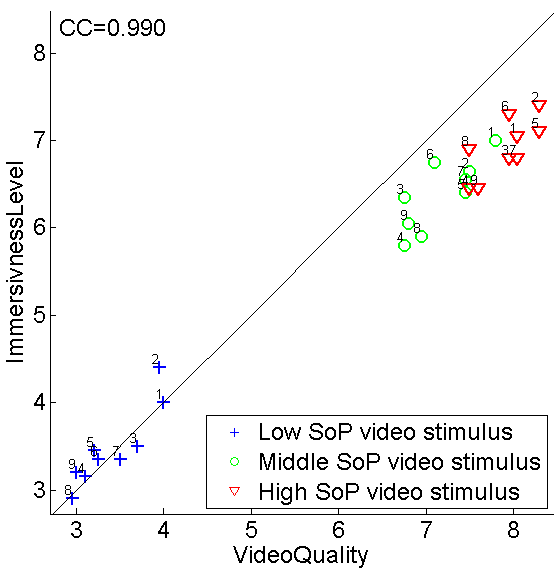
\includegraphics[width=0.3\textwidth]{./images/VA_IL_C.png}
    \caption{Correlation between the experienced \ac{SoP} and the assessed quality of the video }
    \label{Correlation}
\end{figure}

Figure \ref{Correlation} depicts the correlation between the \ac{MOS} rates given for the video quality and the \ac{SoP}. Each sequence is identified by a number, allowing the study of the assessment evolution depending on the \ac{IL} of a sequence.
The correlation coefficient of \ac{IL} and video quality is 0.99, meaning that these two characteristics are highly correlated. A huge difference is observed between the low class and middle/high class, corroborating with the previous analysis. It should be pointed out that each sequence provides a better immersive experience when its \ac{IL} is increased.


\begin{table}[h]
\resizebox{0.57\textwidth}{!}{
\begin{minipage}{0.7\textwidth}
\begin{tabular}{ |m{2cm} | m{1cm} m{2cm} m{2cm} m{1.6cm} | }
   %\hline	
   %frequency band of EEG features  \\
   \hline	
   		 	& video quality		& Interest in video content 	& Interest in audio content		& Surrounding awareness \\
   \hline	
   Immersiveness level 				& 0.990		& 0.914		& 0.974		& -0.986 \\
   video quality 					& 	-		& 0.892		& 0.988		& -0.987 \\
   Interest in video content 		& 	-		& 	-		& 0.857		& -0.903 \\
   Interest in audio content 		& 	-		& 	-		& 	-		& -0.965 \\
   \hline	
 \end{tabular}
\caption[caption]{Pearson correlation coefficients between the ratings of different \\ perceptual aspects }
\label{OC}
\end{minipage} }
\end{table}

The table \ref{OC} confirms the high correlation between \ac{IL} and the video quality (cc = 0.99), and shows the influence to having sound or not (cc = 0.97). It also valid that the surrounding awareness is inversely related with the \ac{IL} (cc ~= -0.99).


\subsection{Physiological signal analysis}
This section presents the pre-processing steps to remove the artifacts, the feature extraction methods and the classification results.

\subsubsection{Pre-processing}
The manually rejection of muscle activity related \ac{EEG} electrodes leads to a total of 216 electrodes for processing and analysis. \ac{EEG} signals were filtered between 3-47 Hz using a third-order Butterworth filter, in order to remove \ac{EOG}and \ac{EMG} artifacts.
[TO SET : DENOISING FUNCTION]

\ac{ECG} signals were used to extract the \ac{HRV}, which reflects the sympathetic/parasympathetic modulation. \ac{HRV} is the physiological measurement of variation in the time interval between consecutive hearts beats.\\
In order to extract the \ac{HRV}, the interval between two QRS complexes defined as R-R interval ($t_{R-R}$)was estimated using the real-time algorithm developed by Pan and Tompkins \cite{HR}. Then the heart rate (HR, in beats per minute) was estimated as :
\begin{equation}
	HR = \frac{60}{t_{R-R}}
\end{equation}

The \ac{HRV} is the variation of HR over time. As the HR is a time-series of non-uniform R-R intervals, the HR was regularly resampled at 4 Hz rate.
[TO SET : respiration denoising]

Both respiratory signals (abdomen and thoracic) were filtered by a wavelet multivariate de-noising
\cite{waveletDenoise}.
It combines univariate wavelet de-noising in the basis where the estimated noise covariance matrix is diagonal and non-centered Principal Component Analysis (PCA) on approximations in the wavelet domain.

In the presented results, only 19 \ac{EEG} signals were kept to expedite the validation of the database.


\subsubsection{Feature extraction}
[He?]
\subsubsection{Classification}
[He?]

\subsubsection{Results}
[Me]


 
\section{Conclusion}


\bibliographystyle{abbrv}
\bibliography{sigproc} 

\end{document}
